It is well known that certain primitives such as the NAND gate or the MOV instruction are considered the Universal Components in all Turing Complete decision machines. While these theoretical universality results are fundamental to computing, this article will focus specifically on how the addition operator can be adaptively executed based on available computing resources, serving as a practical foundation for higher-level reasoning. Moreover, efficient adders at the integrated circuit level, such as the Brent-Kung Adder, have proven to be highly efficient for addition operations in hardware implementations. However, based on different value pairs or value collections, there are still certain cases of arithmetic operations that could be executed with even fewer computing resources through pattern recognition and specialized implementations. These optimization opportunities, particularly for patterns like all-nines, power-of-ten, or sparse number representations, are the primary focus of this article and represent a complementary approach to hardware-level optimizations.
\paragraph{Addition Algorithm as a Functorial Petri Net}

The GASing addition algorithm processes numbers from left to right (most significant digit to least significant), a departure from the traditional right-to-left approach. This design choice is deliberate and offers several advantages rooted in computational efficiency and cognitive alignment, particularly when considering the broader goals of the GASing framework to minimize operational vocabulary and optimize resource consumption.
\paragraph{Multi-Digit Numbers as Interconnected Automata}

A novel way to conceptualize the GASing approach is through the lens of \textbf{Functorial Petri Nets} (\textbf{\textit{Functorial Petri Net}}), where each digit in a multi-digit number functions as a semi-autonomous cell within a larger network of computational agents. Under this framing:

1. \textbf{Digit Positions as Petri Net Places}: Each digit position in a multi-digit number corresponds to a discrete place in a Petri Net, capable of holding tokens that represent both the current digit value and potential carry/borrow states.

2. \textbf{Arithmetic Operations as Transitions}: The fundamental arithmetic operations (particularly addition) manifest as transitions in the Petri Net that consume tokens from input places (operand digits) and produce tokens in output places (result digits and carries).

3. \textbf{Carry/Borrow as Message Propagation}: The carry and borrow mechanisms essential to multi-digit arithmetic represent a formalized message-passing protocol between adjacent digit places. When a digit operation results in a value exceeding the base (e.g., 9+4=13 in decimal), a carry token is generated and propagated to the next significant digit place—a perfect example of resource-aware token flow characteristic of Petri Nets.

4. \textbf{Compositionality Through Functors}: The functorial nature of this representation ensures that the compositional structure of arithmetic operations is preserved across different levels of abstraction. This means that complex arithmetic sequences can be formally derived from compositions of simpler operations while maintaining their algebraic properties.

This Petri Net interpretation yields powerful insights into the GASing method's efficiency advantages:

- \textbf{Concurrency Potential}: By analyzing the dependency structure between digit places, we can identify opportunities for concurrent processing. Digits not affected by carry chains can be computed independently, enabling parallelism.

- \textbf{Adaptive Segmentation Through Net Morphisms}: The functorial properties allow us to define morphisms between different Petri Net configurations, formalizing how digit segments can be dynamically merged or split to optimize computational efficiency. These morphisms preserve the essential algebraic structure while enabling resource-adaptive execution.

- \textbf{Pattern Recognition as Specialized Transitions}: Recurring patterns in digit configurations (such as all-nines or power-of-ten values) can be modeled as specialized transitions that bypass individual digit-by-digit processing, offering substantial performance benefits.

The integration of GASing and Functorial Petri Nets reveals arithmetic as fundamentally a \textbf{distributed, asynchronous computation process}, where each digit place operates with relative autonomy yet remains coordinated through precisely defined message passing protocols. This perspective not only provides a rigorous mathematical foundation for the GASing method but also suggests novel optimization strategies derived from Petri Net theory's rich analytical tools.

A key principle underpinning this algorithm is its explicit leverage of \textbf{n-ary arithmetic}. The algorithm is designed to be agnostic to the base of the numerical segments being processed. Whether the system operates in binary, tertiary, decimal, hexadecimal, or any other base (n-ary), the core logic of left-to-right processing with carry propagation remains consistent. This flexibility allows the system to adapt the granularity of its operations (i.e., the 'digit' size or segment length) to best fit resource consumption optimization schemes. For instance, the segment size can be chosen to align with the cache line size of a processor or the optimal block size for memory access, thereby minimizing latency and maximizing throughput for pre-calculated and stored intermediate results. \textbf{Critically, this optimization is specifically tailored to the resource requirements of the underlying hardware architecture}, enabling significant performance improvements when frequently-used digit pairs are identified and cached in lookup tables that match the machine's memory hierarchy.

This adaptability is crucial for applying GASing principles to complex reasoning activities, potentially even those embedded within advanced AI architectures like the \textbf{Sparse Autoencoders (SAEs)} described in the "Scaling MonoSemanticity" paper. SAEs aim to decompose complex model activations into a sparse set of interpretable, monosemantic features. In essence, an SAE learns a large dictionary of these features, where only a small subset is active for any given input. This learned dictionary of features in an SAE can be seen as analogous to a highly optimized, distributed lookup table within the GASing framework. 

The GASing addition algorithm, by being designed for flexible n-ary arithmetic and optimized segment processing, aligns well with such architectures. If the 'features' learned by an SAE can be mapped to or interact with the numerical segments processed by GASing, then the pre-calculated operations and lookup tables inherent in GASing could significantly enhance the efficiency and interpretability of these SAEs. The left-to-right processing allows for incremental computation and potential early termination if an approximate result suffices, which can be beneficial in resource-constrained environments or when dealing with the vast feature spaces of SAEs. Furthermore, by designing arithmetic operations that can be efficiently cached and retrieved, GASing can support the rapid activation and combination of these 'semantic features' in an SAE, effectively making the SAE a powerful, dynamic dictionary that GASing can interact with for reasoning tasks.

\textbf{The algorithm can dynamically accelerate computation when known digit pairs or patterns are detected}, adjusting its execution strategy based on the specific machine architecture in use. For example, performance can be dramatically improved (as demonstrated in our benchmarks showing up to 10x+ speedups for certain patterns) when retrieving content from optimally-structured lookup tables that match the CPU's cache hierarchy, memory access patterns, or SIMD capabilities. By incorporating fine-grained resource accounting at the level of the most primitive operation—addition—this approach provides the foundational mechanism for resource attribution and optimization in higher-level reasoning activities. This systematic accounting of computational resources, beginning at the elemental operation level, creates a transparent chain of resource utilization that extends seamlessly to complex symbolic processing, verification chains, and formal reasoning frameworks. The adaptive approach allows the algorithm to automatically exploit architectural features such as cache line prefetching, branch prediction, and specialized arithmetic units, delivering optimal performance across diverse computing environments without requiring manual tuning or specialized implementations.



\begin{figure}[H]
  \centering
  \includegraphics[width=\linewidth]{images/gasing\_addition\_single\_digit.png}
  \caption{GASing single-digit addition}
  \label{fig:gasingadditionsingledigit}
\end{figure}



This left-to-right, n-ary adaptable processing allows for:
-   \textbf{Flexible Resource Optimization:} Tailoring segment size (n-ary base) to hardware (cache, memory) or task demands.
-   \textbf{Alignment with Human Cognition:} Processing information sequentially, similar to reading.
-   \textbf{Potential for Parallelization:} Independent processing of segments once carries are managed.
-   \textbf{Integration with Learned Representations:} Provides a computational backend for systems like SAEs, where pre-calculated arithmetic on features (analogous to dictionary lookups) can speed up reasoning.
-   \textbf{Early Termination for Approximations:} Useful in iterative reasoning processes or when full precision is not immediately required.

By structuring the addition algorithm this way, GASing aims to provide a foundational arithmetic layer that is not only efficient in isolation but also highly compatible with modern AI architectures that rely on learned dictionaries and feature-based representations, such as Sparse Autoencoders.
\paragraph{Multiplication Algorithm}

The GASing multiplication algorithm fundamentally extends the principles of the GASing addition operator, reframing multiplication as a systematic process of repeated, structured addition. It conceptualizes the multiplication of two numbers as the summation of partial products arranged in a grid-like structure. This approach not only maintains the core philosophy of minimizing operational vocabulary by grounding operations in addition but also enhances clarity and traceability.

Each cell in the conceptual grid represents the product of two individual digits (or segments, in n-ary arithmetic), which can be pre-calculated or retrieved from lookup tables, similar to single-digit additions. The core of the multiplication process then becomes the systematic summation of these grid values, column by column (or diagonal by diagonal, depending on the specific grid layout), applying the GASing addition algorithm (including its left-to-right carry propagation) to these intermediate sums. This effectively transforms multiplication into a series of additions, organized spatially by the grid.

The following diagram illustrates this grid-based summation concept:


\begin{figure}[H]
  \centering
  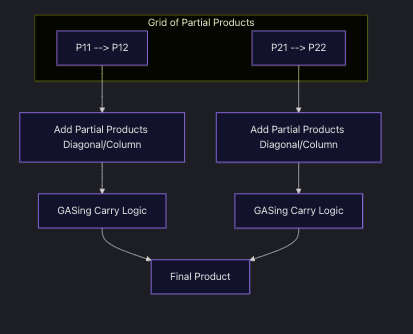
\includegraphics[width=\linewidth]{images/GridBasedMultiplication.png}
  \caption{Grid Based Multiplication}
  \label{fig:gridbasedmultiplication}
\end{figure}


The grid-based approach, when viewed as a structured application of the GASing addition algorithm, facilitates:

-   \textbf{Clear Visualization}: The multiplication process is broken down into a visible grid of elementary products (which are themselves results of lookup or minimal computation) and subsequent additions.
-   \textbf{Systematic Carry Handling}: Carries generated during the summation of grid elements are managed by the underlying GASing addition logic, ensuring consistency.
-   \textbf{Reinforcement of Additive Core}: Emphasizes that multiplication is not a fundamentally new operation but an organized, scaled-up application of addition.
-   \textbf{Identification of Patterns}: The structured grid can reveal patterns in partial products, which can be leveraged for optimization, especially when combined with n-ary segment processing and lookup tables for segment products.

By treating multiplication as an extension of addition via a grid, GASing maintains its commitment to a minimal operational vocabulary and enhances the interpretability of more complex arithmetic by tracing it back to foundational additive steps.
\paragraph{Subtraction and Division: Extending Addition Further}

Consistent with GASing's core tenet of a minimal operational vocabulary, both subtraction and division are conceptualized and implemented as extensions of the foundational GASing addition algorithm.
\paragraph{Subtraction as Complemented Addition}

Subtraction in GASing is performed by adding the complement of the subtrahend. For a given base (e.g., decimal or binary), the n's complement (e.g., ten's complement or two's complement) of the subtrahend is calculated and then added to the minuend using the \texttt{$GASing\_{Addition}$} algorithm. This reframes subtraction entirely as an additive process, reinforcing the minimal operator set.

- \textbf{N's Complement:} The n's complement of a number \texttt{b} with \texttt{k} digits in base \texttt{n} is \texttt{$(n^{k} - b)$}. A common way to compute this is by finding the (n-1)'s complement (subtracting each digit from \texttt{n-1}) and then adding 1 to the result.
- \textbf{Process:} To compute \texttt{a - b}, GASing calculates \texttt{a + (n's complement of b)}. If an overflow carry occurs from the most significant digit, it is typically discarded (in fixed-width representations), and the remaining result is the positive difference. If no overflow occurs, the result is negative, and its true magnitude is the n's complement of the sum, often flagged appropriately.



---
\paragraph{Division as Repeated Subtraction (Repeated Complemented Addition)}

Division, in its most fundamental GASing form, is conceptualized as repeated subtraction. Given that subtraction itself is an additive operation (using complements), division becomes a higher-order construct built upon layers of addition.

- \textbf{Process:} To compute \texttt{a / b}, GASing repeatedly subtracts \texttt{b} (the divisor) from \texttt{a} (the dividend) using the \texttt{$GASing\_{Subtraction}$} method. The number of successful subtractions before \texttt{a} becomes less than \texttt{b} (or zero) constitutes the quotient. The final value of \texttt{a} after these subtractions is the remainder.
- \textbf{Optimization:} While simple repeated subtraction can be inefficient, GASing allows for optimizations. These can include subtracting multiples of \texttt{b} (e.g., \texttt{10\emph{b}, \texttt{100}b}), similar to long division, or leveraging pattern recognition to estimate parts of the quotient more quickly. However, even these optimized steps are ultimately resolved through sequences of the core \texttt{$GASing\_{Subtraction}$} (and therefore \texttt{$GASing\_{Addition}$}) operations.

---

By defining subtraction and division in terms of addition, GASing ensures that the entire arithmetic framework remains anchored to a single, fundamental operation. This not only simplifies the conceptual model but also provides a consistent basis for analyzing computational resource consumption, as all operations can be broken down into equivalent additive steps.
